
\section{Technique}
\label{sec:approach}

This section first explains \ourtool's 3 steps, as introduced
in Section~\ref{sec:introduction} and illustrated
in Figure~\ref{fig:workflow}; and then gives \ourtool's full algorithm
in Section~\ref{sec:algorithm}


\begin{figure*}[t]
  \centering
  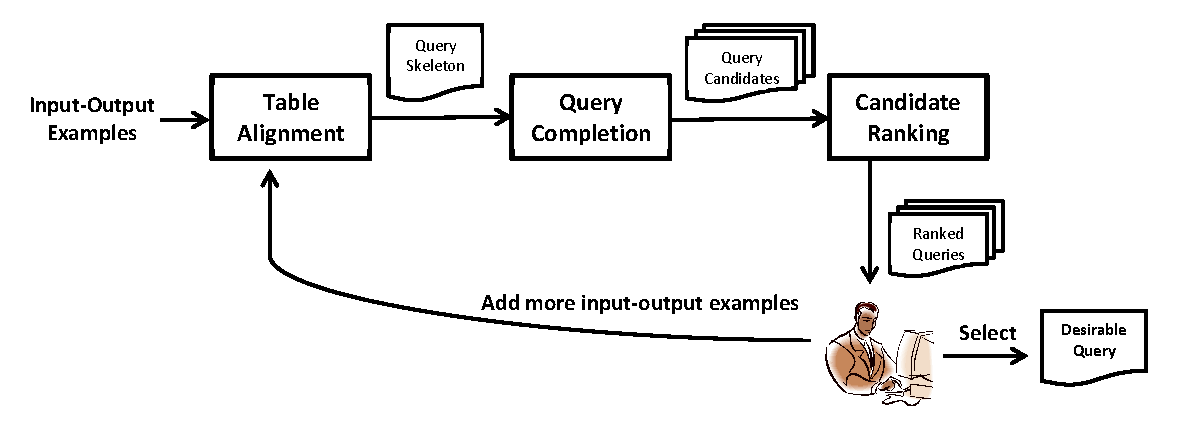
\includegraphics[scale=0.70]{workflow}
  \vspace*{-1.0ex}\caption {{\label{fig:workflow} Illustration
  of \ourtool's workflow in inferring SQL queries from input-output examples. \ourtool consists of 3 steps: (1) The ``Skeleton Creation'' step (Section~\ref{sec:skeleton})
infers a partially-complete SQL query as a skeleton from the given
examples, (2) The ``Query Completion'' step (Section~\ref{sec:completion}) uses
a rule-learning algorithm~\cite{} and type-directed search to
produces a list of syntactically-valid query candidates that satisfy
the provided input-output examples.
, and (3) The ``Candidate Ranking'' step (Section~\ref{sec:ranking})
ranks all inferred SQL query candidates and provides users a
ranked list of SQL queries with the likely ones on the top. 
Users select the
desirable SQL queries from the produced ranked query list. On some
examples, if \ourtool produces SQL queries that satisfy the input and
output examples, but does not address the intention that the user wants;
\ourtool can be used interactively by asking users to provide more
informative examples and then refine the SQL queries.
}}

\end{figure*}


\subsection{Query Skeleton Creation}
\label{sec:skeleton}

%\todo{why need a skeleton. We divide the whole inference
%into three tasks}


A query skeleton is a partially-complete SQL query.
It consists of three parts: the tables used in
the query, the table columns used to join tables, and the table
columns used to project the query results.
Other elements in the query, such as query conditions
and aggregate functions, will be determined in
the next step.

A query skeleton captures the most basic structure of
a SQL query; creating it is the first step of sythesizing
a complete query. \ourtool performs a simple scan over
the examples, and employs several heuristics to determine
the table set, joining columns, and project columns.

\todo{why heuristics. the source of PSPACE}

%\item
\vspace{1mm}
{\textbf{Determining the Table Set.}} 
We observe that End-users are often unwilling to provide more than enough
input: every table in the example input
is expected to be used (at least once) in the result query.
Thus, we assume that every input table
should be used in the query. 
%By default, the table set contains all given input tables.
On the other hand, it is possible that one input table will be
used for multiple times in a query.
\ourtool does not forbid this case,
rather, it uses a heuristic
to estimate the table set: if one column from
an input table appears multiple times in the
example output, we add the input table to the table set the same
number of times.\todo{xx}

The rationale behind this heuristic is that if a table column
appears multiple times in the output, it may indiciate that the
table would be joined multiple times.



%\item
\vspace{1mm}
%\noindent
{\textbf{Determining the Joining Columns. }} Given a set of tables,
there are many ways to join them. Enumerating all possibilities
leads to a huge number of joining conditions and would quickly
become intractable. To make it feasible, we use
three simple but effective effective rules to capture
the most likely ways to join tables in practice.
%based We observe that, in practice, two tables are
%often joined via the following
%three cases: 
First, tables are often joined on their primary keys with
the same data type. For example, in Figure~\ref{fig:motivating},
the \CodeIn{student} table can be joined with the \CodeIn{enrolled}
table on the \CodeIn{student\_id} column.
By contrast, it is unlikely to join two tables on columns
with different types. Second, tables are often joined
on columns with the same name, since columns with the same name
often such as joining the \CodeIn{student} table
with the \CodeIn{enrolled} table on the
\CodeIn{student\_name} column. Third, it is only meaningful
to join two tables on columns that have the same data type and some
overlapped values. \todo{revise}

\ourtool restricts the search space in uses the above three rules \todo{need to revise}

%It is straightforward to check the first 
%two cases to identify possible joining columns. For the third case, our technique scans the given input tables to check ``value similarity''
%between two arbitrary columns, and selects columns whose ``value similarity'' is above a fixed threshold as joining columns.
\todo{need to implement above.}
\todo{mention how many skeletons will be created}
\todo{give an algorithm}

%\item
%\vspace{1mm}
%\noindent 
{\textbf{Determining the Output Columns.}} For each
column in the output table, \ourtool first checks whether
its column name appears in any of the input table.
If so, \ourtool uses the matched column from the input
table as the output column.
Otherwise, the output column
must be produced by using an aggregate function.
\todo{same names}
Consider the example in Figure~\ref{fig:motivating},
\ourtool determines that column {\CodeIn{name}} comes from the \CodeIn{student}
table, while column {\CodeIn{max\_Score}} must be created by using an aggregation operator.
\todo{If there is no column name}
%which the querying result would be projected, our technique checks whether each output
%table column name appears in any input tables. If so, we used the matched column
%from the input table as the output column.  Our technique keeps track of those aggregation columns
%and search for proper aggregates in the next phase (Section~\ref{sec:agg_search}). 
\todo{check the values in the output column}

\todo{It is possible that multiple skeleton can be created. add an algorithm here.}
\vspace{1mm}




\begin{figure}[t]
	\centering
		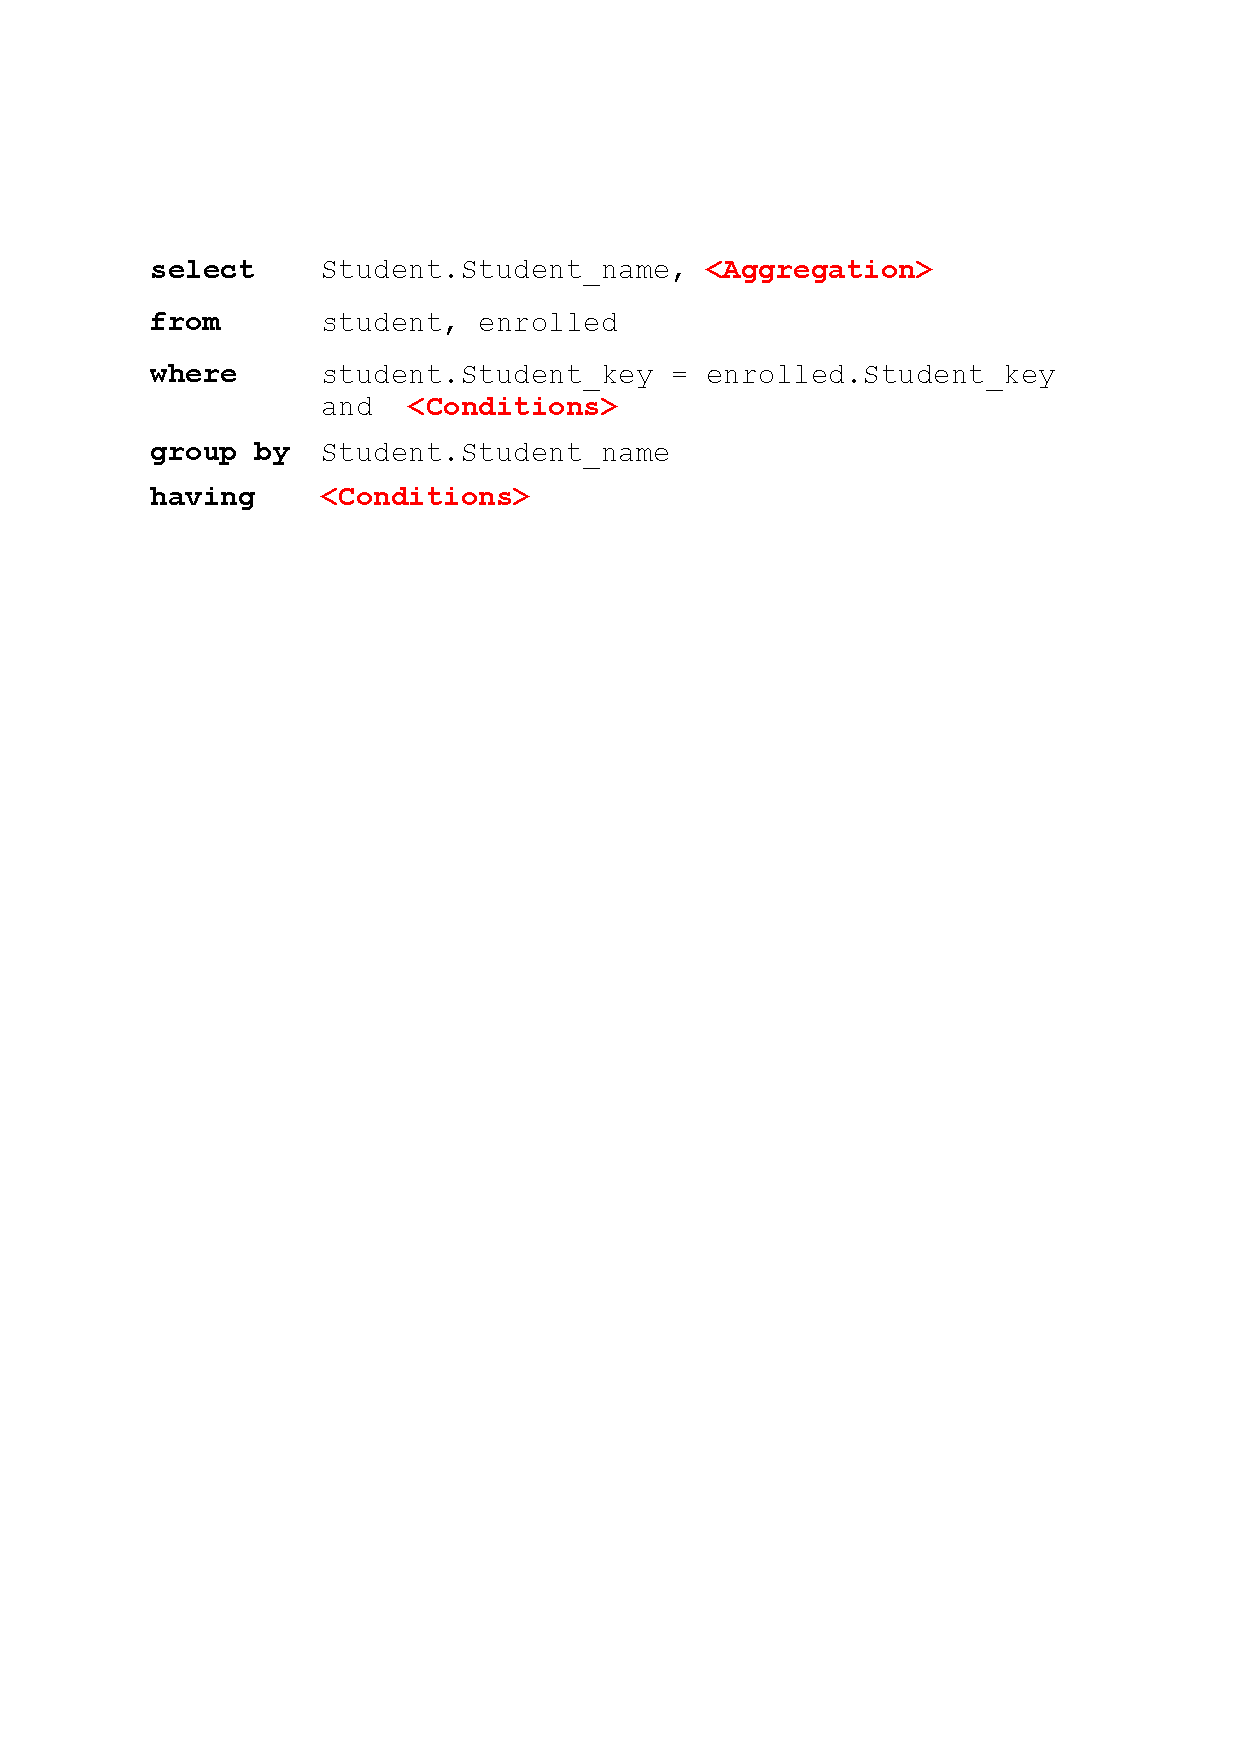
\includegraphics[width=0.45\textwidth]{sql_skeleton.pdf}
	\caption{The SQL skeleton created for the motivating example
in Figure~\ref{fig:motivating}.}
	\label{fig:skeleton}
\end{figure}

Figure~\ref{fig:skeleton} shows the created query skeleton
for the motivating example in Figure~\ref{fig:motivating}.
In this skeleton,  three unknown structures represented by
$<$Aggregation$>$ or $<$Conditions$>$ are in red, and
will be filled in the next phase. \todo{revise text}


\todo{how to create group by}

% which indicates aggregation and group by.

%After determining the table set and joining columns,
%the next step is to identify potential column names on which the result would be projected. If a
%column in the output table  does not appear in any input table's column list, this output column must
%be produced by aggregation. Our algorithm keeps track of these columns and appends a \CodeIn{group by} ... \CodeIn{having} ...
%clause to the query skeleton.

%\end{itemize}

%In summary, this step infers three parts as a query skeleton: tables used in constructing a SQL query, joining conditions
%to connect the input tables, and a list of columns to project the output results.

%It is worth noting that the results obtained from the above steps are not \textit{safe} in
%terms that they may miss some valid SQL queries. 

%We made the above assumption for the sake of tractability,
%since in theory, the bound of table number in a SQL query is $O(n_t!)$, where $n_t$ is the number of given tables;
%while the bound of possible number of join is $O(c_t^2)$ and the bound of the number of conditions is $O(n_t!n_tc_t^2)<O(n_t^3c_t^2)$.

%\subsubsection{Inferring Output Table Schema}

%Lacks schema


%while the bound of possible number of join is $O(c_t^2)$ and the bound of the number of conditions is $O(n_t!n_tc_t^2)<O(n_t^3c_t^2)$.




\subsection{Query Completion}
\label{sec:completion}

\begin{figure*}[t]
    \centering
    \includegraphics[scale=0.68]{featurex}
    \vspace{-7mm}
	\caption{Illustration of the two additional features
    added by \ourtool. (Left) An example input table with
    two columns: C1 and C2. (Center) The aggregation features added by
    \ourtool for the input table. (Right) The comparison features
    added by \ourtool for the input table.
    Take the first row in the input table as an example,
    when grouping by column C1 (with value 2), the number
    of tuples falling into that group is 3; the 
    distinct values in the C2 column is 2; the minimal value
    in the C2 column is 1, the maximal value in the C2 column
    is 4, and the average value in the C2 column is 2. Similarl
    results can be computed when the table is grouped by the C2
    column.
}
	\label{fig:features}
\end{figure*}


In this step, \ourtool analyzes each created query skeleton
, and completes the missing query conditions, the
\CodeIn{GROUP BY} and \CodeIn{HAVING} clause (Section~\ref{sec:condition}),
aggregates (Section~\ref{sec:agg_search}), and
the \CodeIn{ORDER BY} clause (Section~\ref{sec:orderby}).
\ourtool outputs a list of syntactically-correct SQL queries
that satisfy the given example input and output.


%The SQL skeleton produced by the first step, though incomplete,
%serves as a good reference in inferring complete and valid SQL queries.
%In this step, our technique the remaining incomplete parts: conditions and
%aggregates, by rule-based learning and type-directed search, respectively.

\subsubsection{Inferring Query Conditions}
\label{sec:condition}

\ourtool casts the problem of \textit{inferring query conditions} as
 \textit{learning appropriate rules} that can perfectly divide a search space
into a positive part and a negative part. In our context, the search space
is all tuples from joining all query tables; the positive part
includes all tuples in the output table; and the negative part includes the rest
tuples.

The standard way for rule learning is using a decision-tree-based
algorithm. However, how to design a good features
becomes a key challenge.
Existing approaches~\cite{Tran:2009} simply use
tuple values in the input table(s) as features, 
and limits their abilities in inferring more
complex rules as query conditions. In particular,
merely using tuple values as features can only infer
conditions that compares a column value with a constant
(e.g., \CodeIn{student.level = 'senior'}), but
fails to infer conditions using aggregates (e.g., \CodeIn{COUNT(enrolled.course\_id) > 2}),
or conditions comparing the values of two table columns
(e.g., \CodeIn{enrolled.course\_id > enrolled.score}).



\ourtool addresses this challenge by adding two types of
additional features to each tuple, and uses
the existing tuple values together with the additional features
for rule learning.

\begin{itemize}

\item {\textbf{Aggregation Features}}. For each
column in an input table, \ourtool tries
to group all table data by \textit{each} tuple's
value, then applies every applicable aggregate (i.e.,
\CodeIn{COUNT}, \CodeIn{COUNT DISTINCT}, \CodeIn{MAX},
\CodeIn{MIN}, and \CodeIn{AVG} for a numeric type column;
and \CodeIn{COUNT}, and \CodeIn{COUNT DISTINCT} for
a string type column) to every
 \textit{remaining} column for computing the aggregation result. 
The ``Aggregation Features'' part in Figure~\ref{fig:features}
shows an example.

\item {\textbf{Comparison Features}}. For each tuple,
\ourtool compares
the values of every two type-comparable columns, and records
the comparison results ($1$ or $0$) as features.
The ``Comparison Features'' part in Figure~\ref{fig:features}
shows an example.

\end{itemize}

%The above two additional features seamlessly encodes SQL
%structure
% knowledge encoding permits our technique
%to make use of correlations between columns, rather than only values
%from each isolated and sequential columns.
%Table~\ref{tbl:com} shows an example.


%Using both tuple values and the enhanced features,
\ourtool employs a variant of the decision tree algorithm,
called PART~\cite{Frank:1998}, to learn a set of rules
as query conditions.
PART has two notable advantages over the
original decision tree algorithm~\cite{Quinlan:1986}.
First, it uses a ``divide-and-conquer'' strategy to repeatedly
build rules and remove data instances (i.e., tuples) that have already been covered until
no more data instances are left, and thus is faster.
Second, PART less memory, since it builds a decision
tree incrementally, prunes falsified branches on-the-fly,
and only keeps the minimal tree structure in memory.



\todo{The incerasing number of features, can be falsified quickly,
more features permits undiscover more rules}


Figure~\ref{fig:fullexample} shows an example, in
which the expected query condition uses the \CodeIn{COUNT} aggregate.


\begin{figure*}[t]
  \centering
  \includegraphics[scale=0.65]{fullexample}
  \vspace*{-5.0ex}\caption {{\label{fig:fullexample}
  Illustration of how additional features added by \ourtool
  helps in inferring query conditions. (a) shows \ourtool
  enriches the original table (Left: the
  result of joining table \CodeIn{student} with table
  \CodeIn{enrolled} on the \CodeIn{student\_id} column)
  with additional features. For brevity, only relevant
  aggregation features are shown. Using the added aggregation
  features, \ourtool infers two query conditions that
  transform the original table into the table show in (b).
  Note that, without the aggregation features enhanced by
  \ourtool, a learning algorithm will \textit{fail} to learn the above conditions.
  (c) shows the output table, which is produced by projecting the
   table in (b)
  on its column: name, and an aggregate: \CodeIn{MAX}(score).
}}

\end{figure*}


\ourtool next splits the learnt rules into two disjoint parts:
and put each part into its appropriate place.
Specifically, \ourtool puts conditions
using aggregates to the \CodeIn{HAVING}
clause; and puts other conditions to the \CodeIn{WHERE} clause.
This is based on the SQL language's specification:
query conditions using aggregates are valid only when they
are used \textit{after} the \CodeIn{GROUP BY} clause.
Take the conditions inferred in Figure~\ref{fig:fullexample}
as an example, \ourtool puts the query
condition: \CodeIn{student.level =`senior'}
in the \CodeIn{WHERE} clause,
puts condition: \CodeIn{COUNT(enrolled.course\_id) > 2}
in the \CodeIn{HAVING} clause, and puts
column \CodeIn{student\_id} to the \CodeIn{GROUP BY} clause.

%\smallskip





%\end{itemize}

\subsubsection{Searching for Aggregates}
\label{sec:agg_search}

For every column in the output table that has no matched
column in the input tables,
\ourtool repeatedly applies each aggregate on
every input table column; and then outputs the aggregate (with the
input table column) that produces the same output 
in the output table. To speed up the exhaustive search,
\ourtool uses two rules to filter away many infeasible
combinations.


\begin{itemize}
\item \ourtool only applies an \textit{applicable} aggregate
to a \textit{type-compatible} table column. Specifically,
the data values in an output column must be compatible with an
aggregator's return type. For instance, if an output column
contains float values, it cannot be produced by using the \CodeIn{COUNT}
or \CodeIn{COUNT DISTINCT} aggregators, or 
using the \CodeIn{MAX} aggregator over a column with integer type.
On the other hand, some aggregates cannot be applied on
table columns with certain types. For example, the \CodeIn{AVG}
aggregate cannot be applied to columns with string type.
%\ourtool encodes such knowledge to avoid unnecessary search.

\item \ourtool checks whether each value in the output
column has appeared in the input table. If not, the
output column cannot be produced by using
using the \CodeIn{MAX} and \CodeIn{MIN} aggregator.
%such as \CodeIn{MAX} and \CodeIn{min},
%is used, each value in the output column must has appeared in the input table.
\end{itemize}

%In our experience, the type-directed searching strategy significantly reduces the
%searching space and makes our tool find the desirable aggregates faster.

%\todo{Order by structure, relatively each to add}
\subsubsection{Searching for columns in the \CodeIn{ORDER BY} column}
\label{sec:orderby}
\ourtool scans the values of each column in the output table. If
the data values in a column are sorted, \ourtool
append the column name to the \CodeIn{ORDER BY} clause.


\subsection{Candidate Ranking}
\label{sec:ranking}


It is possible that multiple SQL queries satisfying
the given input-output examples will be returned.
This may adversely impact end-users who want to
perform simple query tasks but now need
to select the query of their intent.
To alleviate this problem, we employ
the Occam's razor principle, which states that the
simplest explanation is usually the correct one, to
rank a more likely query higher in the output list.
A simpler query is less likely to overfit the given examples
than a complex query, even when both of them
can transform the example input to the example output.


%We define a comparison scheme between different
%SQL queries by defining a partial order between them. Some of
%these choices are subjective, but have been observed to work well.
A SQL query is simpler than another one if it uses
fewer query conditions (including conditions in the \CodeIn{Having}
and \CodeIn{from} clauses) or the expressions (including
aggregates) in each query condition are pairwise simpler
(e.g., expression \CodeIn{Count(student\_id)} is simpler than
\CodeIn{Count(Distinct student\_id)}.
Simpler query conditions suggests the extraction logics
are more common and general.

In our implementation, \ourtool computes a cost for each
query, and prefers queries with lower costs. The cost
for a SQL query is computing approximately by summarizing
the number of conditions, aggregates,
and other expressions
appearing in the \CodeIn{group by} and \CodeIn{order by} clauses.
This heuristic, though fairly simple, has been observed
to work well.
Figure~\ref{fig:rank} shows an example.


\begin{figure}[t]
\centering
 \includegraphics[scale=0.80]{rankexample}
 \vspace{-3mm}
\Caption{{\label{fig:rank} Illustration of \ourtool's
query candidate ranking heuristic. \ourtool produces two
queries for the given input-output examples. Based on
the heuristic in Section~\ref{sec:ranking}, the first query
differs from the second query by using simpler conditions,
and thus is ranks higher.
}}
\end{figure}



\subsection{Overview}
\label{sec:algorithm}

\vspace{-1mm}

Figure~\ref{fig:workflow} illustrates \ourtool's workflow.
\ourtool consists of three steps: (1) the ``Skeleton Creation'' step (Section~\ref{sec:skeleton})
creates a set of query skeletons from the given examples;
(2) the ``Query Completion'' step (Section~\ref{sec:completion}) 
infers the missing parts in each query skeleton and outputs
a list of syntactically-valid queries that satisfy
the provided example input and output; and (3) the ``Candidate Ranking'' step (Section~\ref{sec:ranking})
ranks all synthesized SQL queries and places the more likely ones near the top. 
Users can inspect the query list and select an expected query
from it.
If the synthesized SQL queries satisfy the example input and
output, but do not address the user's intention,
\ourtool can be used interactively by requesting more
informative examples from the end-user and then
update the result queries.\todo{xx}

Take the query in Figure~\ref{fig:queryex} as an example,
the ``Skeleton Creation''
step infers its projection columns, query tables, and join conditions; and
the ``Query Completion'' step infers the remaining parts (i.e., aggregates,
query conditions, the \CodeIn{GROUP BY} clause, the
\CodeIn{HAVING} clause, and the \CodeIn{ORDER BY} clause).

Figure~\ref{fig:algorithm} sketches \ourtool's high-level algorithm.
Line 2 corresponds to the first ``Query Skeleton
Creation'' step. Lines 3 -- 13 correspond to the second ``Query Completion''
step, in which \ourtool searches for the query conditions (line 4)\footnote{
Including conditions used in the \CodeIn{HAVIGN} clause.},
aggregates (line 5), and columns in the \CodeIn{ORDER BY} clause (line 6).
\ourtool then assembles a list of candidate SQL queries (line 7), and
validates their correctness on the examples (lines 8 -- 11).
Line 14 corresponds to the ``Query Ranking'' step.

%the result list (line 10). Finally, the query list is sorted by using
%the Occam's razor principle (line 14), and returned to the end-users.

\begin{figure}[t]

\textbf{Input}: example input table(s) $T_I$, example output table $T_O$\\

\vspace{-4mm}
\textbf{Output}: a ranked list of SQL queries\\
\vspace{1mm}
synthesizeSQLQueries({$T_{I}$, $T_{o}$})\\
\vspace{-5mm}
\begin{algorithmic}[1]
\STATE $\mathit{queryList}$ $\leftarrow$ an empty list\\
\STATE $\mathit{skeletons}$ $\leftarrow$ createQuerySkeletons($\mathit{T_I}$, $\mathit{T_O}$)
\FOR{each $\mathit{skeleton}$ in $\mathit{skeletons}$}
\STATE $\mathit{conds}$ $\leftarrow$ inferConditions($\mathit{T_I}$, $\mathit{T_O}$, $\mathit{skeleton}$)
\STATE $\mathit{aggs}$ $\leftarrow$ searchForAggregates($\mathit{T_I}$, $\mathit{T_O}$, $\mathit{skeleton}$, $conds$)
\STATE $\mathit{columns}$ $\leftarrow$ searchForOrderBys($\mathit{T_O}$, $\mathit{skeleton}$, $\mathit{aggs}$)
\STATE $\mathit{queries}$ $\leftarrow$ buildQueries($\mathit{skeleton}$, $\mathit{conds}$, $\mathit{aggs}$, $\mathit{columns}$)
\FOR{each $\mathit{query}$ in $\mathit{queries}$}
\IF{isValidOnExamples($\mathit{query}$, $\mathit{T_I}$, $\mathit{T_O}$)}
\STATE $\mathit{queryList}$.add($\mathit{query}$)
\ENDIF
\ENDFOR
\ENDFOR
\STATE rankQueries($\mathit{queryList}$)
\RETURN $\mathit{queryList}$
\end{algorithmic}
\vspace{-3mm}
\caption{Algorithm for synthesizing SQL queries from input-output examples.}
 \label{fig:algorithm}
\end{figure}


\subsection{Discussion}
\label{sec:uim}

We next discuss some design issues in \ourtool.

\noindent \textbf{Soundness and Completeness.} The \ourtool
technique is neither sound nor complete. The primary
reason is that the Query Skeleton Creation step (Section~\ref{sec:skeleton})
in \ourtool is based on heuristics.
\todo{such heuristics approximate the NP hard problems.}
Thus, \ourtool cannot gurantee to infer correct SQL queries
in all cases. Despite such limitations,
as demonstrated in Section~\ref{sec:evaluation}, \ourtool
is still useful in sythesizing many SQL queries in practice.

\vspace{1mm}
\noindent \textbf{What if the input-output examples are not
representative enough?}
On some examples, \ourtool may produce a SQL query that
satisfies the input-output examples specified by the user,
but does not address the intention that the user wants.
To address this issue, we use a simple
interaction model~\cite{Harris:2011} to ask users to
investigate the results of an output SQL query and report any discrepancy.
After, the user can refine the inferred SQL query by providing a more
informative input-output example that demonstrate the behavior on
which the originally-inferred SQL query behaves incorrectly.
As demonstrated in our evaluation (Section~\ref{sec:evaluation}),
such an interactive model works well in practice: \todo{a
few interations}




